% !TEX TS-program = pdflatex
% !TEX encoding = UTF-8 Unicode

% This is a simple template for a LaTeX document using the "article" class.
% See "book", "report", "letter" for other types of document.

\documentclass[11pt]{article} % use larger type; default would be 10pt

\usepackage[utf8]{inputenc} % set input encoding (not needed with XeLaTeX)
\usepackage{lscape,amsmath}
%%% Examples of Article customizations
% These packages are optional, depending whether you want the features they provide.
% See the LaTeX Companion or other references for full information.

%%% PAGE DIMENSIONS
\usepackage{geometry} % to change the page dimensions
\geometry{a4paper} % or letterpaper (US) or a5paper or....
% \geometry{margins=2in} % for example, change the margins to 2 inches all round
% \geometry{landscape} % set up the page for landscape
%   read geometry.pdf for detailed page layout information
\usepackage{multicol,multirow,array}
\usepackage{graphicx} % support the \includegraphics command and options

% \usepackage[parfill]{parskip} % Activate to begin paragraphs with an empty line rather than an indent

%%% PACKAGES
\usepackage{booktabs} % for much better looking tables
\usepackage{array} % for better arrays (eg matrices) in maths
\usepackage{paralist} % very flexible & customisable lists (eg. enumerate/itemize, etc.)
\usepackage{verbatim} % adds environment for commenting out blocks of text & for better verbatim
\usepackage{subfig} % make it possible to include more than one captioned figure/table in a single float
% These packages are all incorporated in the memoir class to one degree or another...

%%% HEADERS & FOOTERS
\usepackage{fancyhdr} % This should be set AFTER setting up the page geometry
\pagestyle{fancy} % options: empty , plain , fancy
\renewcommand{\headrulewidth}{0pt} % customise the layout...
\lhead{}\chead{}\rhead{}
\lfoot{}\cfoot{\thepage}\rfoot{}

%%% SECTION TITLE APPEARANCE
\usepackage{sectsty}
\allsectionsfont{\sffamily\mdseries\upshape} % (See the fntguide.pdf for font help)
% (This matches ConTeXt defaults)

%%% ToC (table of contents) APPEARANCE
\usepackage[nottoc,notlof,notlot]{tocbibind} % Put the bibliography in the ToC
\usepackage[titles,subfigure]{tocloft} % Alter the style of the Table of Contents
\renewcommand{\cftsecfont}{\rmfamily\mdseries\upshape}
\renewcommand{\cftsecpagefont}{\rmfamily\mdseries\upshape} % No bold!

%%% END Article customizations

%%% The "real" document content comes below...

\title{Brief Article}
\author{The Author}
%\date{} % Activate to display a given date or no date (if empty),
         % otherwise the current date is printed 

\begin{document}
\noindent Caitlin McHugh\\
Oct 2014 \\ 

\noindent I simulated 500 SNPs for 100 iterations of a 16-person pedigree for a total of 1,600 samples.
The SNPs varied in frequency, with 100 SNPs each at the following frequencies: 0.01, 0.05, 0.1, 0.2, 0.25. 


\begin{figure}[hb]
\centering
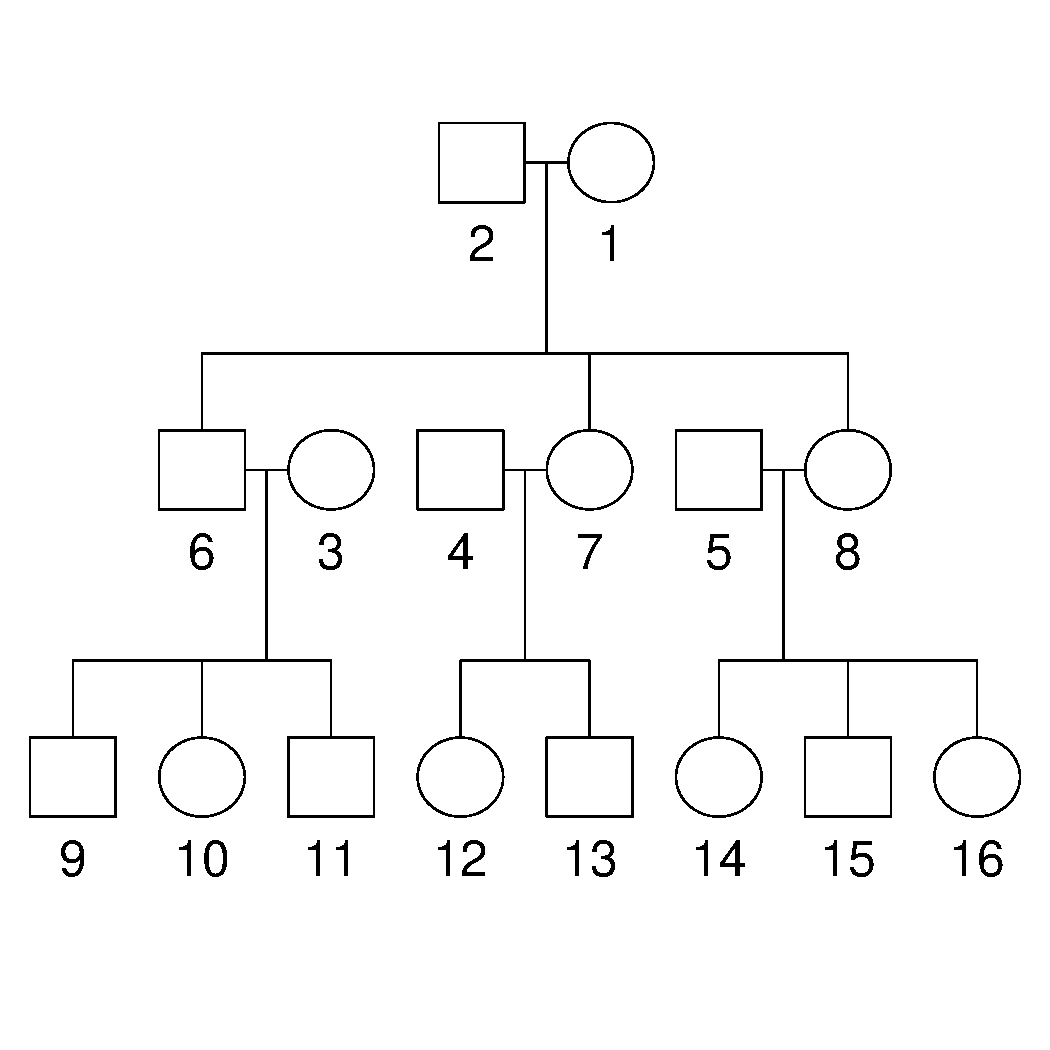
\includegraphics[height=7cm]{pedigree_16individs.pdf}
\caption{The 16-person pedigree used for the simulations.}
\end{figure}


I estimated the variance components for the autosomes and the X chromosome, using the true kinship matrix in both cases.
I then fit the mixed model for a quantitative trait on the X chromosome, testing the genotypes simulated on the X chromosome.

\begin{table}[ht]
\centering
\begin{tabular}{rrrrr}
  \hline
  &$\alpha$=1e-04& $\alpha$=5e-04 & $\alpha$=0.001 & $\alpha$=0.01 \\ 
  \hline
auto + X adj & 0.00000 & 0.00043 & 0.00144 & 0.01249 \\ 
auto adj & 0.00047 & 0.00217 & 0.00347 & 0.02405 \\ 
X adj & 0.00000 & 0.00040 & 0.00150 & 0.01326 \\ 
   \hline
\end{tabular}
\caption{Type I error rate for 5,000 independent simulations of 6 different parameter combinations for 30,000 total simulation runs.}
\end{table}

\begin{table}[ht]
\centering
\begin{tabular}{rrrrr}
  \hline
  &$\alpha$=1e-04& $\alpha$=5e-04 & $\alpha$=0.001 & $\alpha$=0.01 \\ 
  \hline
auto + X adj& 0.00000 & 0.00016 & 0.00128 & 0.01288 \\ 
auto adj & 0.00012 & 0.00202 & 0.00314 & 0.02429 \\ 
X adj & 0.00000 & 0.00012 & 0.00136 & 0.01385 \\ 
   \hline
\end{tabular}
\caption{Type I error rate as above but excluding SNPs with a MAF$\leq$0.01 for a total of 25,770 simulations.}
\end{table}

\begin{table}[ht]
\centering
\begin{tabular}{rrrrrr}
  \hline
 $\beta_1$ & $h^2$ & p & $\sigma^2_A$ & $\sigma^2_X$ & $\sigma^2_E$ \\ 
  \hline
0.04366 & 0.010 & 0.2 & 0.1 & 5 & 1 \\ 
 0.10919 & 0.025 & 0.2 & 0.1 & 5 & 1 \\ 
 0.21858 & 0.050 & 0.2 & 0.1 & 5 & 1 \\ 
0.43881 & 0.100 & 0.2 & 0.1 & 5 & 1 \\ 
 0.89122 & 0.200 & 0.2 & 0.1 & 5 & 1 \\ 
 1.03186 & 0.230 & 0.2 & 0.1 & 5 & 1 \\ 
   \hline
\end{tabular}
\caption{Parameters for the 6 different scenarios considered for the simulation runs.}
\end{table}

\begin{figure}
\centering
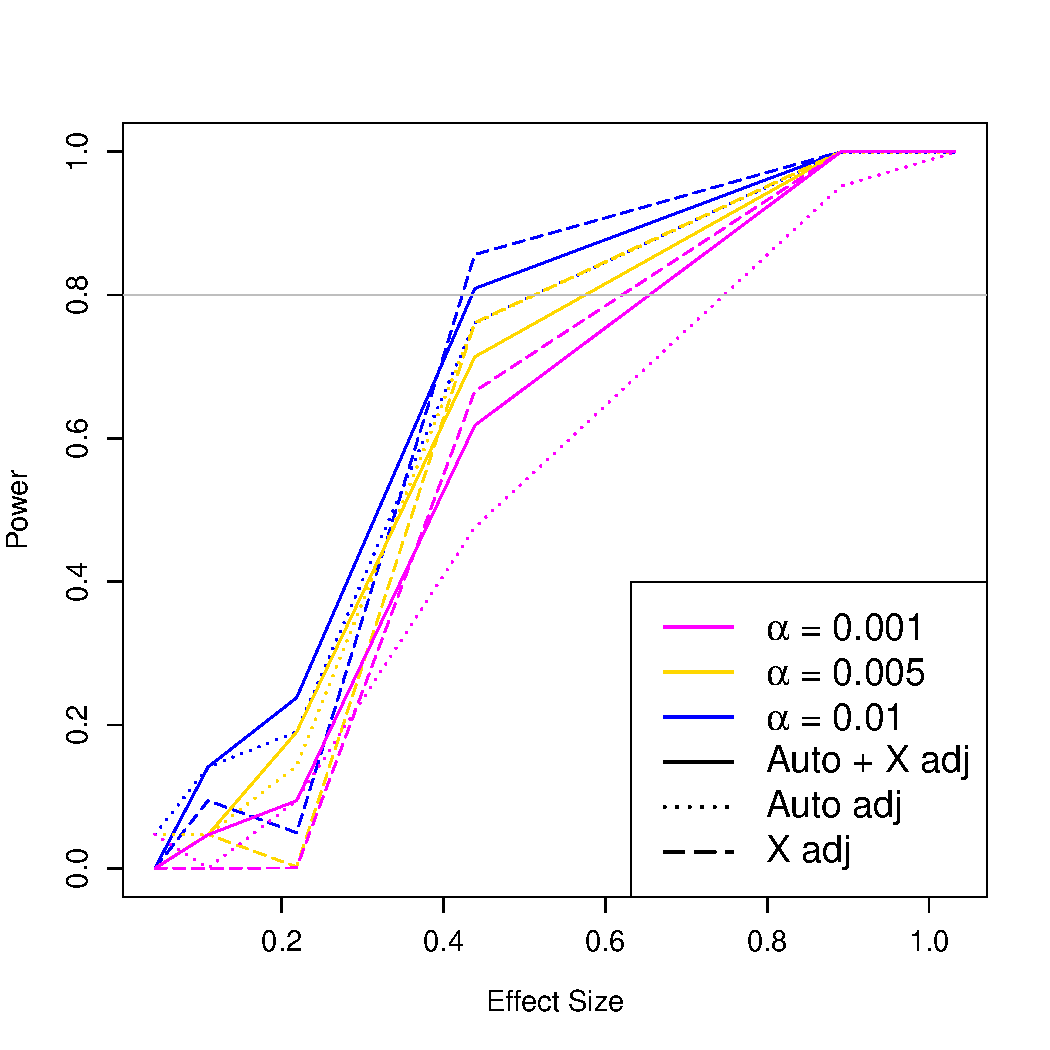
\includegraphics[height=14cm]{powerRes_10000Iters.pdf}
\caption{Power results for mixed models that either include or exclude adjustment for X chromosome kinship. 
Three values of $\alpha$ are considered for 10,000 independent iterations each.}
\end{figure}


\bgroup
\def\arraystretch{1.5}
\begin{table}[ht]
\centering
\begin{tabular}{crcc}
  \hline
&& Autosomes & X Chromosome\\
  \hline
&Mother-Daughter &$\frac{1}{2}$ & $\frac{1}{2}$\\
&Mother-Son, Father-Daughter &$\frac{1}{2}$& $\frac{\sqrt{2}}{2}$\\
%&Father-Daughter &$\frac{1}{2}$&$\frac{\sqrt{2}}{2}$\\
&Father-Son &$\frac{1}{2}$&0\\
&Full sisters & $\frac{1}{2}$ & $\frac{3}{4}$\\
&Full brothers &$\frac{1}{2}$&$\frac{1}{2}$\\
&Sister-Brother &$\frac{1}{2}$&$\frac{\sqrt{2}}{4}$\\
\hline
\parbox[t]{2mm}{\multirow{8}{*}{\rotatebox[origin=c]{90}{\Large{Maternal}}}} & Aunt-Niece &$\frac{1}{4}$&$\frac{6}{16}$\\
&Aunt-Nephew&$\frac{1}{4}$&$\frac{3\sqrt{2}}{8}$\\
&Uncle-Niece &$\frac{1}{4}$&$\frac{\sqrt{2}}{8}$\\
&Uncle-Nephew &$\frac{1}{4}$&$\frac{1}{4}$\\
&Grandma-Granddaughter &$\frac{1}{4}$&$\frac{1}{4}$\\
&Grandma-Grandson &$\frac{1}{4}$&$\frac{\sqrt{2}}{4}$\\
&Grandpa-Granddaughter&$\frac{1}{4}$&$\frac{\sqrt{2}}{4}$\\
&Grandpa-Grandson &$\frac{1}{4}$&$\frac{1}{2}$\\
\hline
\parbox[t]{2mm}{\multirow{8}{*}{\rotatebox[origin=c]{90}{\Large{Paternal}}}} &Aunt-Niece &$\frac{1}{4}$&$\frac{1}{4}$\\
&Aunt-Nephew&$\frac{1}{4}$&0\\
&Uncle-Niece &$\frac{1}{4}$&0\\
&Uncle-Nephew &$\frac{1}{4}$&0\\
&Grandma-Granddaughter &$\frac{1}{4}$&$\frac{1}{2}$\\
&Grandma-Grandson &$\frac{1}{4}$&0\\
&Grandpa-Granddaughter&$\frac{1}{4}$&0\\
&Grandpa-Grandson &$\frac{1}{4}$&0\\
   \hline
\end{tabular}
\caption{The theoretical genetic relatedness (GR) values stratified by X chromosome and autosomes. The autosomal GR value is twice the kinship coefficient $= 2(\frac{1}{2}\kappa_2+\frac{1}{4}\kappa_1)$, where $\kappa_1$ and $\kappa_2$ are the probabilities of sampling one and two alleles IBD, respectively. The X chromosome GR value for male-male pairs is $\kappa_1$, the probability of sampling one allele IBD. Female-female pairs yield an X chromosome GR value of twice $\kappa_1$ as calculated on the X chromosome. For female-male pairs, the X chromosome GR value is $\sqrt{2}\kappa_1$.}
\end{table}

\newpage
The genetic relatedness (GR) values were calculated using equations presented in (GCTA software paper) and are the following:
\begin{align}
GR(X_j,X_k)&=\frac{1}{N}\sum^N_i \frac{(X_{ij}-2p_i)(X_{ik}-2p_i)}{2p_i(1-p_i)} \\
GR(X_j,X_l)&=\frac{1}{N}\sum^N_i \frac{(X_{ij}-2p_i)(X_{il}-p_i)}{\sqrt{2}p_i(1-p_i)}\\
GR(X_l,X_m)&=\frac{1}{N}\sum^N_i \frac{(X_{il}-p_i)(X_{im}-p_i)}{p_i(1-p_i)}
\end{align}
where $X_j$ and $X_k$ are females and $X_l$ and $X_m$ are males.


\newpage
I simulated 500 SNPs for 100 iterations of a 16-person pedigree for a total of 1,600 samples with some relatedness structure, plus 500 unrelated samples (250 males, 250 females). 
There are a total of 5 founders per pedigree * 100 pedigrees + 500 unrelateds = 1,000 unrelated samples in this set.

The model we assume when testing for association on X chromosome SNPs is 
\begin{align}
y &= \beta_0 + \beta_1 \mbox{SNP}_x + g_A + g_X +\epsilon \\
g_A &\sim MVN(0,\sigma^2_A \Phi_A) \\
g_X &\sim MVN(0,\sigma^2_X \Phi_X) 
\end{align}
where SNP$_x$ is the genotype vector of a SNP on the X chromosome that is being tested for association, $\Phi_A$ is the genetic relatedness matrix as measured on the autosomes and $\Phi_X$ is the genetic relatedness matrix on the X chromosome.

We can calculate the variance for a given individual $i$ to be the sum of the variances of the SNP being tested, the variance due to X chromosome, autosomes and environment (or error)
\begin{align}
var(y_i)&=\beta_1^2 2p(1-p)+\sigma^2_A +\sigma^2_\epsilon + \sigma^2_X
\end{align}

The parameter of $h^2_{snp}$ can be calculated from the equation
\begin{align}
h^2_{snp}&=\frac{\beta_1^2 2p(1-p)}{\beta_1^2 2p(1-p)+\sigma^2_\epsilon + \sigma^2_A + \sigma^2_X}
\end{align}
where $p$ is the allele frequency of the causal SNP.
On the other hand, we can calculate the heritability of all SNPs on the X chromosome, which is 
\begin{align}
h^2_{x}&=\frac{\beta_1^2 2p(1-p)+\sigma^2_X}{\beta_1^2 2p(1-p)+\sigma^2_\epsilon + \sigma^2_A + \sigma^2_X}
\end{align}


\bgroup
\def\arraystretch{1.0}
\begin{table}[ht]
\centering
\begin{tabular}{rrrrrr}
  \hline
 Adjustment& $\alpha$=0.01 & $\alpha$=0.005 & $\alpha$=0.001 & $\alpha$=5e-4 & $\alpha$=1e-4 \\ 
  \hline
X  & 0.01343 & 0.00782 & 0.00201 & 0.00115 & 0.00041 \\ 
 Auto  & 0.01503 & 0.00896 & 0.00262 & 0.00163 & 0.00041 \\ 
 X + auto  & 0.01313 & 0.00803 & 0.00211 & 0.00123 & 0.00041 \\ 
   \hline
\end{tabular}
\caption{Type I error for varying heritability and variance values. These were calculated from 119,760 iterations.}
\label{typeIvars}
\end{table}

\newpage
\landscape
\begin{table}[ht]
\centering
\tiny
\begin{tabular}{rrrrrrrr|rrr|rrr|rrr|rrr|rrr}
  \hline
& & & & & & &&\multicolumn{3}{c}{$\alpha=0.01$} & \multicolumn{3}{c}{$\alpha=0.005$} & \multicolumn{3}{c}{$\alpha=0.001$} & \multicolumn{3}{c}{$\alpha=5e-4$}&\multicolumn{3}{c}{$\alpha=1e-4$}\\
$h^2_{x}$& $\beta_1$ & $h^2_{snp}$ & p & $\sigma^2_A$ & $\sigma^2_X$ & $\sigma^2_E$ &sims& X & A & Both &X & A & Both & X &A & Both & X & A & Both & X & A & Both\\ 
  \hline
0.188& 0.022 & 0.010 & 0.2 & 0.3 & 0.3 & 1 & 4990 & 56 & 65 & 46 & 36 & 36 & 36 & 0 & 9 & 0 & 0 & 0 & 0 & 0 & 0 & 0 \\ 
0.143& 0.026 & 0.010 & 0.2 & 0.8 & 0.3 & 1 & 4990 & 13 & 13 & 13 & 11 & 12 & 11 & 0 & 0 & 0 & 0 & 0 & 0 & 0 & 0 & 0 \\ 
 0.381&0.026 & 0.010 & 0.2 & 0.3 & 0.8 & 1 & 4990 & 62 & 65 & 62 & 30 & 23 & 30 & 0 & 9 & 0 & 0 & 9 & 0 & 0 & 0 & 0 \\ 
 0.308&0.029 & 0.010 & 0.2 & 0.8 & 0.8 & 1 & 4990 & 19 & 27 & 19 & 18 & 18 & 18 & 9 & 9 & 9 & 0 & 9 & 0 & 0 & 0 & 0 \\ \hline
0.188&0.056 & 0.025 & 0.2 & 0.3 & 0.3 & 1 & 4990 & 78 & 106 & 79 & 47 & 75 & 47 & 9 & 18 & 9 & 9 & 9 & 9 & 9 & 9 & 9 \\ 
0.143 &0.064 & 0.025 & 0.2 & 0.8 & 0.3 & 1 & 4990 & 55 & 55 & 55 & 19 & 36 & 36 & 0 & 0 & 0 & 0 & 0 & 0 & 0 & 0 & 0 \\ 
0.381&0.064 & 0.025 & 0.2 & 0.3 & 0.8 & 1 & 4990 & 47 & 103 & 56 & 38 & 47 & 38 & 0 & 0 & 0 & 0 & 0 & 0 & 0 & 0 & 0 \\ 
0.308 &0.071 & 0.025 & 0.2 & 0.8 & 0.8 & 1 & 4990 & 40 & 41 & 39 & 9 & 28 & 9 & 9 & 9 & 9 & 9 & 9 & 9 & 0 & 0 & 0 \\ \hline
0.190& 0.112 & 0.050 & 0.2 & 0.3 & 0.3 & 1 & 4990 & 62 & 70 & 61 & 20 & 48 & 20 & 0 & 9 & 0 & 0 & 0 & 0 & 0 & 0 & 0 \\ 
0.145 &0.128 & 0.050 & 0.2 & 0.8 & 0.3 & 1 & 4990 & 71 & 79 & 70 & 42 & 50 & 41 & 9 & 10 & 9 & 9 & 9 & 9 & 0 & 0 & 0 \\ 
0.383&0.128 & 0.050 & 0.2 & 0.3 & 0.8 & 1 & 4990 & 49 & 30 & 49 & 28 & 29 & 28 & 9 & 0 & 9 & 9 & 0 & 9 & 0 & 0 & 0 \\ 
0.309 &0.143 & 0.050 & 0.2 & 0.8 & 0.8 & 1 & 4990 & 117 & 117 & 117 & 47 & 84 & 74 & 27 & 27 & 27 & 9 & 18 & 18 & 9 & 9 & 9 \\ \hline
0.196&0.225 & 0.100 & 0.2 & 0.3 & 0.3 & 1 & 4990 & 67 & 67 & 66 & 47 & 56 & 47 & 0 & 9 & 0 & 0 & 0 & 0 & 0 & 0 & 0 \\ 
0.151&0.258 & 0.100 & 0.2 & 0.8 & 0.3 & 1 & 4990 & 32 & 52 & 33 & 32 & 31 & 31 & 11 & 20 & 20 & 10 & 10 & 10 & 1 & 1 & 1 \\ 
0.387 &0.258 & 0.100 & 0.2 & 0.3 & 0.8 & 1 & 4990 & 24 & 60 & 33 & 13 & 30 & 13 & 1 & 11 & 1 & 0 & 10 & 0 & 0 & 0 & 0 \\ 
0.315 &0.287 & 0.100 & 0.2 & 0.8 & 0.8 & 1 & 4990 & 48 & 57 & 47 & 19 & 38 & 19 & 1 & 1 & 1 & 0 & 1 & 1 & 0 & 0 & 0 \\  \hline
0.220 &0.456 & 0.200 & 0.2 & 0.3 & 0.3 & 1 & 4990 & 34 & 25 & 25 & 22 & 22 & 23 & 19 & 20 & 20 & 19 & 18 & 18 & 0 & 0 & 0 \\ 
0.177 &0.523 & 0.200 & 0.2 & 0.8 & 0.3 & 1 & 4990 & 49 & 48 & 48 & 21 & 34 & 23 & 1 & 11 & 10 & 1 & 10 & 1 & 0 & 0 & 0 \\ 
0.406&0.523 & 0.200 & 0.2 & 0.3 & 0.8 & 1 & 4990 & 197 & 189 & 196 & 138 & 99 & 129 & 30 & 22 & 30 & 3 & 21 & 3 & 1 & 1 & 1 \\ 
0.335&0.582 & 0.200 & 0.2 & 0.8 & 0.8 & 1 & 4990 & 75 & 95 & 66 & 61 & 55 & 63 & 29 & 49 & 30 & 19 & 29 & 29 & 9 & 9 & 9 \\ \hline
0.230 &0.529 & 0.230 & 0.2 & 0.3 & 0.3 & 1 & 4990 & 131 & 152 & 134 & 79 & 83 & 81 & 22 & 23 & 22 & 13 & 12 & 12 & 2 & 2 & 2 \\ 
0.188&0.605 & 0.230 & 0.2 & 0.8 & 0.3 & 1 & 4990 & 142 & 110 & 119 & 70 & 48 & 57 & 28 & 19 & 19 & 19 & 10 & 10 & 9 & 9 & 9 \\ 
0.414& 0.605 & 0.230 & 0.2 & 0.3 & 0.8 & 1 & 4990 & 42 & 75 & 51 & 30 & 31 & 30 & 0 & 1 & 0 & 0 & 1 & 0 & 0 & 0 & 0 \\ 
0.344 &0.674 & 0.230 & 0.2 & 0.8 & 0.8 & 1 & 4990 & 98 & 99 & 89 & 59 & 60 & 58 & 27 & 28 & 28 & 9 & 10 & 9 & 9 & 9 & 9 \\ 
   \hline
&&&&&\multicolumn{3}{r|}{Totals} & 1608 & 1800 & 1573 & 936 & 1073 & 962 & 241 & 314 & 253 & 138 & 195 & 147 & 49 & 49 & 49 \\ 
&&&&\multicolumn{4}{r|}{Type I Error Rates} & 0.013 & 0.015 & 0.013 & 0.0078 & 0.0090 & 0.0080 & 0.0020 & 0.0026 & 0.0021 & 0.0012 & 0.0016 & 0.0012 & 4e-4 & 4e-4 & 4e-4 \\ 
\end{tabular}
\caption{Counts of false postives for varying parameter values, stratified by adjustment for X relatedness, autosomal relatedness, and adjustment for both. Five values of $\alpha$ were considered, although the final two are quite small. The bottom row is the total number of false positives for each column and the corresponding type I error rates averaged across all parameter values considered. These are precisely the values shown in Table~\ref{typeIvars}.}
\end{table}

\end{document}




